我们对于扫地机器人问题,首先实现了 SARSA (State-Action-Reward-State-Action) 算法。
SARSA 是一种基于时间差分(Temporal Difference, TD)的强化学习算法,用于在智能体与环境交互过程中,学习一个状态-动作价值函数(\(Q\) 函数)。它是一个 \textbf{on-policy(依策略)} 的算法,意味着它学习的是当前行为策略下的 \(Q\) 值。

SARSA 的名字来自它更新公式中用到的五个元素:
\begin{itemize}
    \item \(S_t\):当前状态(State)
    \item \(A_t\):当前动作(Action)
    \item \(R_{t+1}\):执行动作后的即时奖励(Reward)
    \item \(S_{t+1}\):下一个状态(State)
    \item \(A_{t+1}\):在下一个状态选择的动作(Action)
\end{itemize}

SARSA 的基本更新公式为:
\[
    Q^{\texttt{new}} \left( s_t, a_t \right) \leftarrow  Q \left( s_t, a_t \right) + \alpha \left[ r_{t} + \gamma Q \left( s_{t+1}, a_{t+1} \right) - Q \left( s_t, a_t \right) \right]
\]
其中,\(\alpha\) 是学习率(learning rate),\(\gamma\) 是折扣因子(discount factor),衡量未来奖励的重要性。\(Q \left( S_t, A_t \right)\) 是状态-动作价值函数。
整个算法可以参考算法~\ref{alg:sarsa}。

\begin{algorithm}[htbp]
\caption{SARSA 算法}\label{alg:sarsa}
\KwIn{学习率 \(\alpha\),折扣因子 \(\gamma\),探索率 \(\epsilon\),训练轮数 \(E\),最大步数 \(T\)}
\KwOut{动作-状态值函数 \(Q(s,a)\)}

初始化 \(Q\) 表为全零矩阵: \(Q(s,a) = \mathbf{0}_{\left|s\right|\times\left|a\right|}\)\;

\For{\( \text{episode} = 1 \) \KwTo \( E \)}{
    初始化环境状态 \( s_0 \)\;
    使用 \(\epsilon\)-greedy 策略,根据当前策略从状态 \(s_t\) 中选择动作 \(a_t\)例如 )\;
    \While{状态 \(s_t\) 不是终止状态 \textbf{or} t < T} {
        执行动作 \(a_t\),观察奖励 \(r_t\) 和下一个状态 \(s_{t+1}\)\;
        利用 \(\epsilon\)-greedy 策略 从状态 \(s_{t+1}\) 根据当前策略选择动作 \(a_{t+1}\)(例如 )\;
         生成随机数 \(p \sim \mathcal{U}(0,1)\)\;

        \eIf{\( p < \epsilon \)}{
            以等概率从动作集合 \( \mathcal{A} \) 中随机选择一个动作 \( a \)\;
        }{
            选择具有最大动作值的动作:\\
            \[ a \leftarrow \arg\max_{a \in \mathcal{A}} Q(s, a); \]
        }
        更新 \(Q\) 表 
        \[Q \left( s_t, a_t \right) \leftarrow  Q \left( s_t, a_t \right) + \alpha \left[ r_{t} + \gamma Q \left( s_{t+1}, a_{t+1} \right) - Q \left( s_t, a_t \right) \right];\]
        
        更新状态与动作
        \[s_t \leftarrow s_{t+1}, \qquad a_t \leftarrow a_{t+1};\]
    }
}
\Return{\( Q(s,a) \)}
\end{algorithm}

\subsection{算法实现细节}

具体实现代码参考附录~\ref{sec:saras}。
此处补充关键实现流程描述:
\begin{itemize}
    \item \textbf{状态映射}:使用 \textsf{state\_to\_index} 函数将二维坐标映射到 \(Q\) 表索引;
    \item \textbf{行为选择}:采取 \(\epsilon\)-greedy 策略在探索与利用之间平衡;
    \item \textbf{SARSA 更新}:在每一步中依据当前动作与下一个动作进行 \(Q\) 值更新;
    \item \textbf{训练结束条件}:达到最大步数或进入终止状态;
    \item \textbf{结果和策略可视化}:使用 matplotlib 绘制学习曲线,展示每轮的平均奖励。并将训练完成后将最终 \(Q\) 表策略渲染为箭头图示。
\end{itemize}

\subsection{实验结果与分析}

在这部分,展示使用 SARSA 方法控制扫地机器人的实验结果,包括策略可视化和学习曲线。

\subsubsection{策略可视化}

通过 \textsf{visualize\_policy\_from\_q} 函数生成的策略图如下所示(见图~\ref{fig:sarsa_policy})。其中箭头方向表示在各状态下的最优动作,我们可以清楚的从策略图中看到智能体能够顺利收集垃圾,获得最好的收益 \(5\),而不是在某些格子处陷入局部最优(获得充电站的收益 \(1\))。

\begin{figure}[htbp] 
    \centering 
    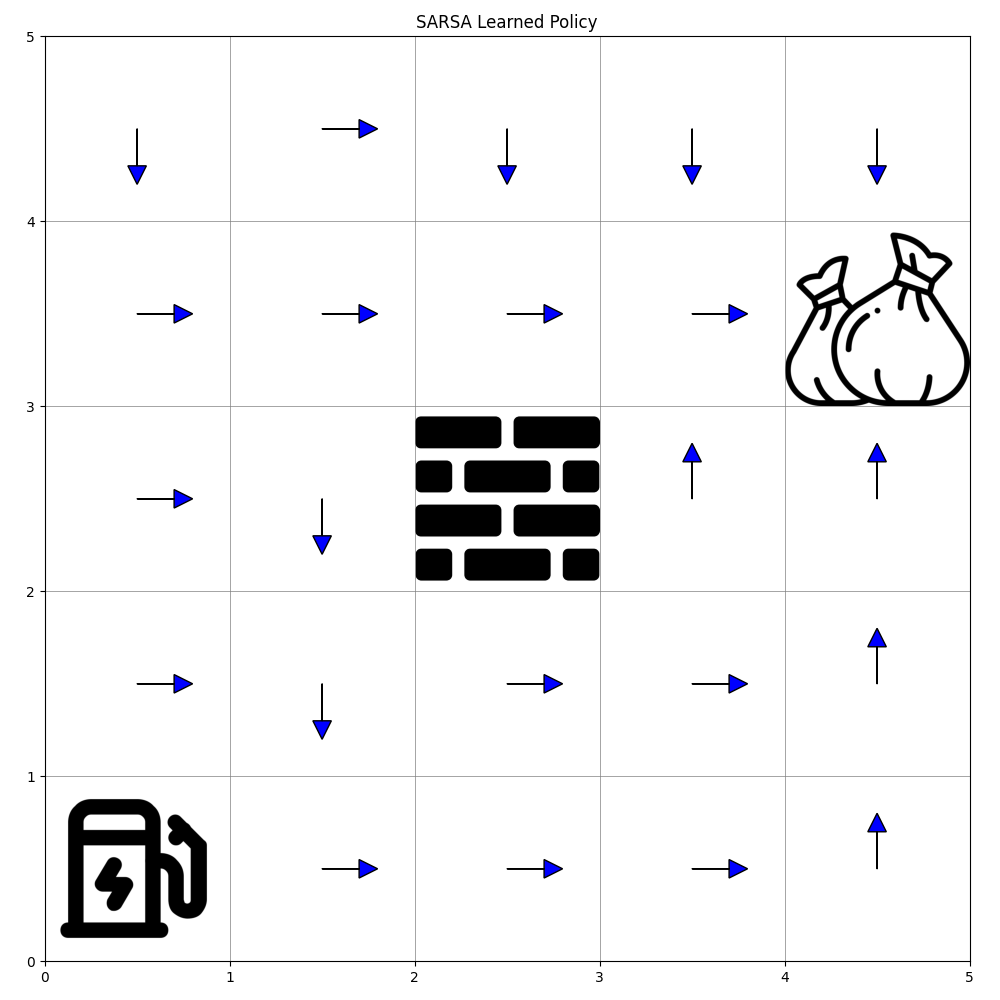
\includegraphics[width=0.5\textwidth]{figure/sweep_robot/sarsa/policy_visualization.png} 
    \caption{SARSA 策略可视化图}\label{fig:sarsa_policy} 
\end{figure}

\subsubsection{学习曲线}

训练过程中的奖励、步数与成功率变化如下图~\ref{fig:sarsa_training} 所示:
其中,我们展示了收益、步数和成功率的变化趋势。
其中我们定义成功率(Success Rate)为机器人成功达到垃圾位置而不是充电站的次数占所有试验次数的比例。
并使用了参数为 \(0.99\) 的指数移动平均值(EMA)进行展示。
可以看到,随着训练的进行,智能体的平均奖励逐渐上升,步数逐渐减少,成功率也在不断提高。这表明智能体逐渐学会了如何在环境中有效地收集垃圾而不是直接去充电站。
初期智能体尝试较多,步数波动较大;后期逐渐收敛。
我们发现成功率呈上升趋势,训练后期趋于稳定,表明智能体学会有效完成任务(捡拾垃圾而不是直接去充电站)。
一开始位置的 \(100\) \% 成功率和总步数为 \(0\) 是因为随机性导致智能体容易直接在垃圾位置附近开始,捡拾成功。

\begin{figure}[htbp] 
    \centering 
    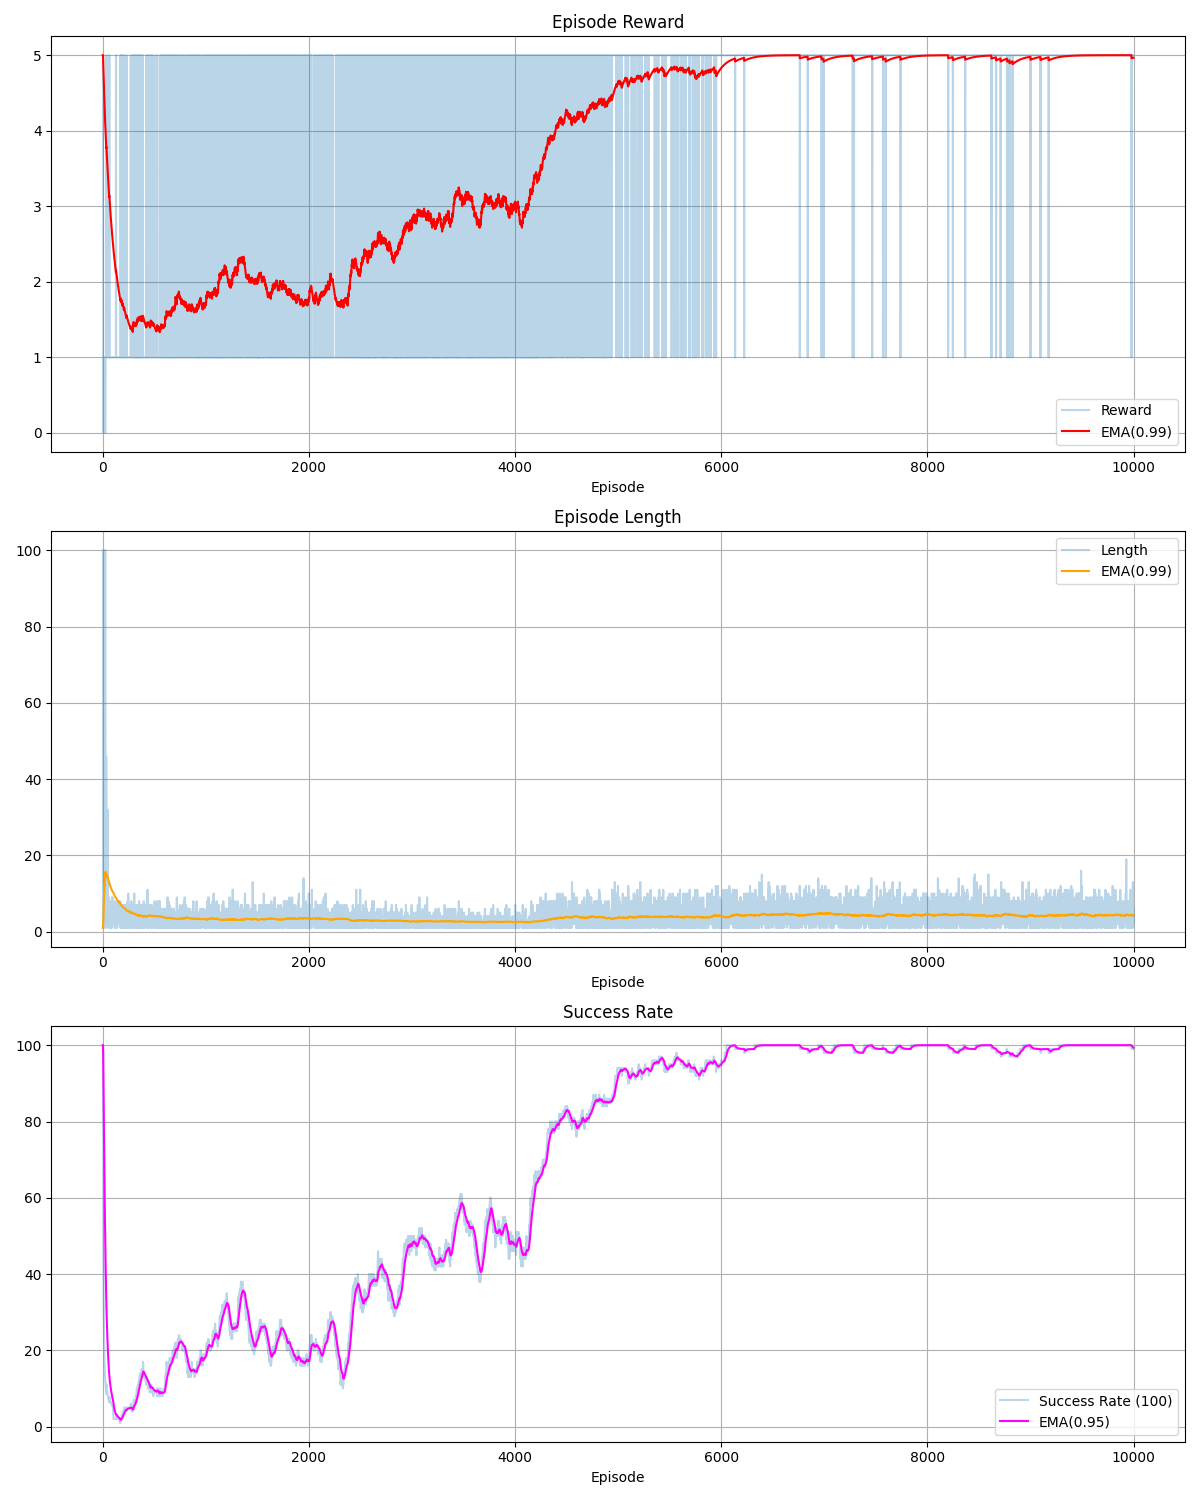
\includegraphics[width=0.8\textwidth]{figure/sweep_robot/sarsa/training_results.png} 
    \caption{SARSA 训练过程统计曲线}\label{fig:sarsa_training} 
\end{figure}

\subsection{参数设置}

本实验中的参数设置如下:
\begin{table}[htbp]
\centering
\caption{SARSA算法主要参数设置}
\label{tab:sarsa_three_line}
\begin{tabular}{ccc}
\toprule
\textbf{参数} & \textbf{取值} & \textbf{说明} \\
\midrule
\(\alpha\)(学习率) & \(0.1\) & 控制每步 \(Q\) 值更新的幅度,决定新经验对旧知识的替代程度。 \\
\(\gamma\)(折扣因子) & \(0.99\) & 衡量未来奖励对当前决策的重要性,越接近 \(1\) 表示越注重长期收益。 \\
\(\epsilon\)(探索率) & \(0.1\) & \(\epsilon\)-贪婪策略中用于随机探索的概率,平衡探索与利用。 \\
总回合数(Episodes) & \(10000\) & 智能体与环境交互的总轮数,较大值有助于收敛策略。 \\
最大步长(per episode) & \(100\) & 每回合允许的最大步数,防止陷入死循环。 \\
\bottomrule
\end{tabular}
\end{table}